% Options for packages loaded elsewhere
\PassOptionsToPackage{unicode}{hyperref}
\PassOptionsToPackage{hyphens}{url}
%
\documentclass[
]{article}
\title{univariate analysis}
\author{}
\date{\vspace{-2.5em}}

\usepackage{amsmath,amssymb}
\usepackage{lmodern}
\usepackage{iftex}
\ifPDFTeX
  \usepackage[T1]{fontenc}
  \usepackage[utf8]{inputenc}
  \usepackage{textcomp} % provide euro and other symbols
\else % if luatex or xetex
  \usepackage{unicode-math}
  \defaultfontfeatures{Scale=MatchLowercase}
  \defaultfontfeatures[\rmfamily]{Ligatures=TeX,Scale=1}
\fi
% Use upquote if available, for straight quotes in verbatim environments
\IfFileExists{upquote.sty}{\usepackage{upquote}}{}
\IfFileExists{microtype.sty}{% use microtype if available
  \usepackage[]{microtype}
  \UseMicrotypeSet[protrusion]{basicmath} % disable protrusion for tt fonts
}{}
\makeatletter
\@ifundefined{KOMAClassName}{% if non-KOMA class
  \IfFileExists{parskip.sty}{%
    \usepackage{parskip}
  }{% else
    \setlength{\parindent}{0pt}
    \setlength{\parskip}{6pt plus 2pt minus 1pt}}
}{% if KOMA class
  \KOMAoptions{parskip=half}}
\makeatother
\usepackage{xcolor}
\IfFileExists{xurl.sty}{\usepackage{xurl}}{} % add URL line breaks if available
\IfFileExists{bookmark.sty}{\usepackage{bookmark}}{\usepackage{hyperref}}
\hypersetup{
  pdftitle={univariate analysis},
  hidelinks,
  pdfcreator={LaTeX via pandoc}}
\urlstyle{same} % disable monospaced font for URLs
\usepackage[margin=1in]{geometry}
\usepackage{color}
\usepackage{fancyvrb}
\newcommand{\VerbBar}{|}
\newcommand{\VERB}{\Verb[commandchars=\\\{\}]}
\DefineVerbatimEnvironment{Highlighting}{Verbatim}{commandchars=\\\{\}}
% Add ',fontsize=\small' for more characters per line
\usepackage{framed}
\definecolor{shadecolor}{RGB}{248,248,248}
\newenvironment{Shaded}{\begin{snugshade}}{\end{snugshade}}
\newcommand{\AlertTok}[1]{\textcolor[rgb]{0.94,0.16,0.16}{#1}}
\newcommand{\AnnotationTok}[1]{\textcolor[rgb]{0.56,0.35,0.01}{\textbf{\textit{#1}}}}
\newcommand{\AttributeTok}[1]{\textcolor[rgb]{0.77,0.63,0.00}{#1}}
\newcommand{\BaseNTok}[1]{\textcolor[rgb]{0.00,0.00,0.81}{#1}}
\newcommand{\BuiltInTok}[1]{#1}
\newcommand{\CharTok}[1]{\textcolor[rgb]{0.31,0.60,0.02}{#1}}
\newcommand{\CommentTok}[1]{\textcolor[rgb]{0.56,0.35,0.01}{\textit{#1}}}
\newcommand{\CommentVarTok}[1]{\textcolor[rgb]{0.56,0.35,0.01}{\textbf{\textit{#1}}}}
\newcommand{\ConstantTok}[1]{\textcolor[rgb]{0.00,0.00,0.00}{#1}}
\newcommand{\ControlFlowTok}[1]{\textcolor[rgb]{0.13,0.29,0.53}{\textbf{#1}}}
\newcommand{\DataTypeTok}[1]{\textcolor[rgb]{0.13,0.29,0.53}{#1}}
\newcommand{\DecValTok}[1]{\textcolor[rgb]{0.00,0.00,0.81}{#1}}
\newcommand{\DocumentationTok}[1]{\textcolor[rgb]{0.56,0.35,0.01}{\textbf{\textit{#1}}}}
\newcommand{\ErrorTok}[1]{\textcolor[rgb]{0.64,0.00,0.00}{\textbf{#1}}}
\newcommand{\ExtensionTok}[1]{#1}
\newcommand{\FloatTok}[1]{\textcolor[rgb]{0.00,0.00,0.81}{#1}}
\newcommand{\FunctionTok}[1]{\textcolor[rgb]{0.00,0.00,0.00}{#1}}
\newcommand{\ImportTok}[1]{#1}
\newcommand{\InformationTok}[1]{\textcolor[rgb]{0.56,0.35,0.01}{\textbf{\textit{#1}}}}
\newcommand{\KeywordTok}[1]{\textcolor[rgb]{0.13,0.29,0.53}{\textbf{#1}}}
\newcommand{\NormalTok}[1]{#1}
\newcommand{\OperatorTok}[1]{\textcolor[rgb]{0.81,0.36,0.00}{\textbf{#1}}}
\newcommand{\OtherTok}[1]{\textcolor[rgb]{0.56,0.35,0.01}{#1}}
\newcommand{\PreprocessorTok}[1]{\textcolor[rgb]{0.56,0.35,0.01}{\textit{#1}}}
\newcommand{\RegionMarkerTok}[1]{#1}
\newcommand{\SpecialCharTok}[1]{\textcolor[rgb]{0.00,0.00,0.00}{#1}}
\newcommand{\SpecialStringTok}[1]{\textcolor[rgb]{0.31,0.60,0.02}{#1}}
\newcommand{\StringTok}[1]{\textcolor[rgb]{0.31,0.60,0.02}{#1}}
\newcommand{\VariableTok}[1]{\textcolor[rgb]{0.00,0.00,0.00}{#1}}
\newcommand{\VerbatimStringTok}[1]{\textcolor[rgb]{0.31,0.60,0.02}{#1}}
\newcommand{\WarningTok}[1]{\textcolor[rgb]{0.56,0.35,0.01}{\textbf{\textit{#1}}}}
\usepackage{graphicx}
\makeatletter
\def\maxwidth{\ifdim\Gin@nat@width>\linewidth\linewidth\else\Gin@nat@width\fi}
\def\maxheight{\ifdim\Gin@nat@height>\textheight\textheight\else\Gin@nat@height\fi}
\makeatother
% Scale images if necessary, so that they will not overflow the page
% margins by default, and it is still possible to overwrite the defaults
% using explicit options in \includegraphics[width, height, ...]{}
\setkeys{Gin}{width=\maxwidth,height=\maxheight,keepaspectratio}
% Set default figure placement to htbp
\makeatletter
\def\fps@figure{htbp}
\makeatother
\setlength{\emergencystretch}{3em} % prevent overfull lines
\providecommand{\tightlist}{%
  \setlength{\itemsep}{0pt}\setlength{\parskip}{0pt}}
\setcounter{secnumdepth}{-\maxdimen} % remove section numbering
\ifLuaTeX
  \usepackage{selnolig}  % disable illegal ligatures
\fi

\begin{document}
\maketitle

\hypertarget{prashanth.s-19mid0020}{%
\section{Prashanth.S 19MID0020}\label{prashanth.s-19mid0020}}

\hypertarget{univariate-analysis}{%
\subsection{Univariate Analysis}\label{univariate-analysis}}

\begin{Shaded}
\begin{Highlighting}[]
\FunctionTok{library}\NormalTok{(plotly)}
\end{Highlighting}
\end{Shaded}

\begin{verbatim}
## Loading required package: ggplot2
\end{verbatim}

\begin{verbatim}
## 
## Attaching package: 'plotly'
\end{verbatim}

\begin{verbatim}
## The following object is masked from 'package:ggplot2':
## 
##     last_plot
\end{verbatim}

\begin{verbatim}
## The following object is masked from 'package:stats':
## 
##     filter
\end{verbatim}

\begin{verbatim}
## The following object is masked from 'package:graphics':
## 
##     layout
\end{verbatim}

\begin{Shaded}
\begin{Highlighting}[]
\FunctionTok{library}\NormalTok{(RColorBrewer)}
\FunctionTok{library}\NormalTok{(ggplot2)}
\FunctionTok{library}\NormalTok{(dplyr)}
\end{Highlighting}
\end{Shaded}

\begin{verbatim}
## 
## Attaching package: 'dplyr'
\end{verbatim}

\begin{verbatim}
## The following objects are masked from 'package:stats':
## 
##     filter, lag
\end{verbatim}

\begin{verbatim}
## The following objects are masked from 'package:base':
## 
##     intersect, setdiff, setequal, union
\end{verbatim}

\begin{Shaded}
\begin{Highlighting}[]
\FunctionTok{library}\NormalTok{(plyr)}
\end{Highlighting}
\end{Shaded}

\begin{verbatim}
## ------------------------------------------------------------------------------
\end{verbatim}

\begin{verbatim}
## You have loaded plyr after dplyr - this is likely to cause problems.
## If you need functions from both plyr and dplyr, please load plyr first, then dplyr:
## library(plyr); library(dplyr)
\end{verbatim}

\begin{verbatim}
## ------------------------------------------------------------------------------
\end{verbatim}

\begin{verbatim}
## 
## Attaching package: 'plyr'
\end{verbatim}

\begin{verbatim}
## The following objects are masked from 'package:dplyr':
## 
##     arrange, count, desc, failwith, id, mutate, rename, summarise,
##     summarize
\end{verbatim}

\begin{verbatim}
## The following objects are masked from 'package:plotly':
## 
##     arrange, mutate, rename, summarise
\end{verbatim}

\hypertarget{diamond-data-set}{%
\subsection{Diamond Data-Set}\label{diamond-data-set}}

\begin{Shaded}
\begin{Highlighting}[]
\NormalTok{df1 }\OtherTok{=}\NormalTok{ diamonds}
\FunctionTok{head}\NormalTok{(df1)}
\end{Highlighting}
\end{Shaded}

\begin{verbatim}
## # A tibble: 6 x 10
##   carat cut       color clarity depth table price     x     y     z
##   <dbl> <ord>     <ord> <ord>   <dbl> <dbl> <int> <dbl> <dbl> <dbl>
## 1  0.23 Ideal     E     SI2      61.5    55   326  3.95  3.98  2.43
## 2  0.21 Premium   E     SI1      59.8    61   326  3.89  3.84  2.31
## 3  0.23 Good      E     VS1      56.9    65   327  4.05  4.07  2.31
## 4  0.29 Premium   I     VS2      62.4    58   334  4.2   4.23  2.63
## 5  0.31 Good      J     SI2      63.3    58   335  4.34  4.35  2.75
## 6  0.24 Very Good J     VVS2     62.8    57   336  3.94  3.96  2.48
\end{verbatim}

\hypertarget{preprocessing}{%
\subsubsection{PreProcessing}\label{preprocessing}}

\begin{Shaded}
\begin{Highlighting}[]
\FunctionTok{cat}\NormalTok{(}\StringTok{"Number of instances  : "}\NormalTok{,}\FunctionTok{nrow}\NormalTok{(df1))}
\end{Highlighting}
\end{Shaded}

\begin{verbatim}
## Number of instances  :  53940
\end{verbatim}

\begin{Shaded}
\begin{Highlighting}[]
\FunctionTok{cat}\NormalTok{(}\StringTok{"}\SpecialCharTok{\textbackslash{}n}\StringTok{Number of attributes : "}\NormalTok{,}\FunctionTok{ncol}\NormalTok{(df1))}
\end{Highlighting}
\end{Shaded}

\begin{verbatim}
## 
## Number of attributes :  10
\end{verbatim}

\begin{Shaded}
\begin{Highlighting}[]
\FunctionTok{str}\NormalTok{(df1)}
\end{Highlighting}
\end{Shaded}

\begin{verbatim}
## tibble [53,940 x 10] (S3: tbl_df/tbl/data.frame)
##  $ carat  : num [1:53940] 0.23 0.21 0.23 0.29 0.31 0.24 0.24 0.26 0.22 0.23 ...
##  $ cut    : Ord.factor w/ 5 levels "Fair"<"Good"<..: 5 4 2 4 2 3 3 3 1 3 ...
##  $ color  : Ord.factor w/ 7 levels "D"<"E"<"F"<"G"<..: 2 2 2 6 7 7 6 5 2 5 ...
##  $ clarity: Ord.factor w/ 8 levels "I1"<"SI2"<"SI1"<..: 2 3 5 4 2 6 7 3 4 5 ...
##  $ depth  : num [1:53940] 61.5 59.8 56.9 62.4 63.3 62.8 62.3 61.9 65.1 59.4 ...
##  $ table  : num [1:53940] 55 61 65 58 58 57 57 55 61 61 ...
##  $ price  : int [1:53940] 326 326 327 334 335 336 336 337 337 338 ...
##  $ x      : num [1:53940] 3.95 3.89 4.05 4.2 4.34 3.94 3.95 4.07 3.87 4 ...
##  $ y      : num [1:53940] 3.98 3.84 4.07 4.23 4.35 3.96 3.98 4.11 3.78 4.05 ...
##  $ z      : num [1:53940] 2.43 2.31 2.31 2.63 2.75 2.48 2.47 2.53 2.49 2.39 ...
\end{verbatim}

\begin{Shaded}
\begin{Highlighting}[]
\FunctionTok{summary}\NormalTok{(df1)}
\end{Highlighting}
\end{Shaded}

\begin{verbatim}
##      carat               cut        color        clarity          depth      
##  Min.   :0.2000   Fair     : 1610   D: 6775   SI1    :13065   Min.   :43.00  
##  1st Qu.:0.4000   Good     : 4906   E: 9797   VS2    :12258   1st Qu.:61.00  
##  Median :0.7000   Very Good:12082   F: 9542   SI2    : 9194   Median :61.80  
##  Mean   :0.7979   Premium  :13791   G:11292   VS1    : 8171   Mean   :61.75  
##  3rd Qu.:1.0400   Ideal    :21551   H: 8304   VVS2   : 5066   3rd Qu.:62.50  
##  Max.   :5.0100                     I: 5422   VVS1   : 3655   Max.   :79.00  
##                                     J: 2808   (Other): 2531                  
##      table           price             x                y         
##  Min.   :43.00   Min.   :  326   Min.   : 0.000   Min.   : 0.000  
##  1st Qu.:56.00   1st Qu.:  950   1st Qu.: 4.710   1st Qu.: 4.720  
##  Median :57.00   Median : 2401   Median : 5.700   Median : 5.710  
##  Mean   :57.46   Mean   : 3933   Mean   : 5.731   Mean   : 5.735  
##  3rd Qu.:59.00   3rd Qu.: 5324   3rd Qu.: 6.540   3rd Qu.: 6.540  
##  Max.   :95.00   Max.   :18823   Max.   :10.740   Max.   :58.900  
##                                                                   
##        z         
##  Min.   : 0.000  
##  1st Qu.: 2.910  
##  Median : 3.530  
##  Mean   : 3.539  
##  3rd Qu.: 4.040  
##  Max.   :31.800  
## 
\end{verbatim}

\hypertarget{bar-chart}{%
\subsubsection{Bar-Chart}\label{bar-chart}}

\begin{Shaded}
\begin{Highlighting}[]
\FunctionTok{table}\NormalTok{(df1}\SpecialCharTok{$}\NormalTok{cut)}
\end{Highlighting}
\end{Shaded}

\begin{verbatim}
## 
##      Fair      Good Very Good   Premium     Ideal 
##      1610      4906     12082     13791     21551
\end{verbatim}

\begin{Shaded}
\begin{Highlighting}[]
\FunctionTok{ggplot}\NormalTok{(df1, }\FunctionTok{aes}\NormalTok{(}\AttributeTok{x=}\FunctionTok{factor}\NormalTok{(cut),}\AttributeTok{fill =} \FunctionTok{factor}\NormalTok{(cut))) }\SpecialCharTok{+}
        \FunctionTok{geom\_bar}\NormalTok{(}\AttributeTok{color=}\StringTok{\textquotesingle{}black\textquotesingle{}}\NormalTok{) }\SpecialCharTok{+} 
        \FunctionTok{labs}\NormalTok{(}\AttributeTok{x =} \StringTok{"Cut"}\NormalTok{, }\AttributeTok{y =} \StringTok{"Count"}\NormalTok{, }\AttributeTok{title  =} \StringTok{"Count of the quality of the Cut"}\NormalTok{)}
\end{Highlighting}
\end{Shaded}

\includegraphics{univariate-analysis_files/figure-latex/unnamed-chunk-7-1.pdf}

\begin{Shaded}
\begin{Highlighting}[]
\FunctionTok{ggplot}\NormalTok{(df1, }
       \FunctionTok{aes}\NormalTok{(}\AttributeTok{x =} \FunctionTok{factor}\NormalTok{(cut), }\AttributeTok{y =}\NormalTok{ ..count.. }\SpecialCharTok{/} \FunctionTok{sum}\NormalTok{(..count..),}\AttributeTok{fill =} \FunctionTok{factor}\NormalTok{(cut))) }\SpecialCharTok{+} 
       \FunctionTok{geom\_bar}\NormalTok{(}\AttributeTok{color=}\StringTok{\textquotesingle{}black\textquotesingle{}}\NormalTok{) }\SpecialCharTok{+}
       \FunctionTok{labs}\NormalTok{(}\AttributeTok{x =} \StringTok{"Cut"}\NormalTok{, }\AttributeTok{y =} \StringTok{"Percentage of Cuts"}\NormalTok{, }\AttributeTok{title  =} \StringTok{"Percentage of the quality of the Cut"}\NormalTok{) }\SpecialCharTok{+}
       \FunctionTok{scale\_y\_continuous}\NormalTok{(}\AttributeTok{labels =}\NormalTok{ scales}\SpecialCharTok{::}\NormalTok{percent)}
\end{Highlighting}
\end{Shaded}

\includegraphics{univariate-analysis_files/figure-latex/unnamed-chunk-8-1.pdf}

\hypertarget{pie-chart}{%
\subsubsection{Pie-Chart}\label{pie-chart}}

\hypertarget{kernel-density-plot}{%
\subsubsection{Kernel Density Plot}\label{kernel-density-plot}}

\begin{Shaded}
\begin{Highlighting}[]
\FunctionTok{ggplot}\NormalTok{(df1, }\FunctionTok{aes}\NormalTok{(}\AttributeTok{x =}\NormalTok{ price)) }\SpecialCharTok{+}
       \FunctionTok{geom\_density}\NormalTok{(}\AttributeTok{fill =} \StringTok{"indianred3"}\NormalTok{) }\SpecialCharTok{+} 
       \FunctionTok{labs}\NormalTok{(}\AttributeTok{title =} \StringTok{"Participants by price"}\NormalTok{)}
\end{Highlighting}
\end{Shaded}

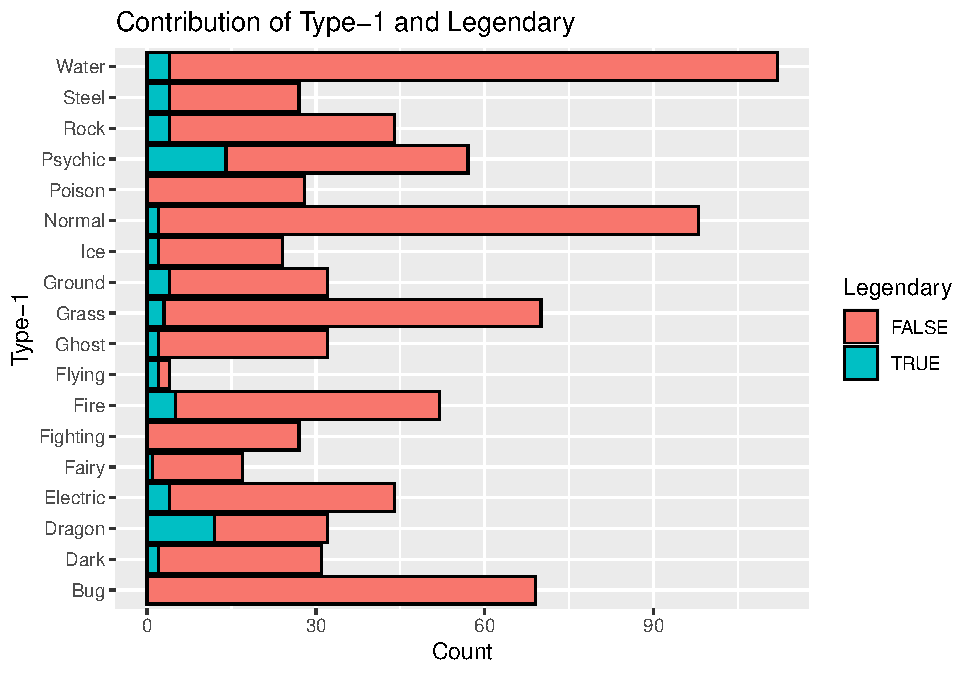
\includegraphics{univariate-analysis_files/figure-latex/unnamed-chunk-10-1.pdf}

\hypertarget{mpg-data-set}{%
\subsection{MPG data-set}\label{mpg-data-set}}

\begin{Shaded}
\begin{Highlighting}[]
\NormalTok{df2 }\OtherTok{=}\NormalTok{ mpg}
\FunctionTok{head}\NormalTok{(df2)}
\end{Highlighting}
\end{Shaded}

\begin{verbatim}
## # A tibble: 6 x 11
##   manufacturer model displ  year   cyl trans      drv     cty   hwy fl    class 
##   <chr>        <chr> <dbl> <int> <int> <chr>      <chr> <int> <int> <chr> <chr> 
## 1 audi         a4      1.8  1999     4 auto(l5)   f        18    29 p     compa~
## 2 audi         a4      1.8  1999     4 manual(m5) f        21    29 p     compa~
## 3 audi         a4      2    2008     4 manual(m6) f        20    31 p     compa~
## 4 audi         a4      2    2008     4 auto(av)   f        21    30 p     compa~
## 5 audi         a4      2.8  1999     6 auto(l5)   f        16    26 p     compa~
## 6 audi         a4      2.8  1999     6 manual(m5) f        18    26 p     compa~
\end{verbatim}

\hypertarget{preprocessing-1}{%
\subsubsection{PreProcessing}\label{preprocessing-1}}

\begin{Shaded}
\begin{Highlighting}[]
\FunctionTok{cat}\NormalTok{(}\StringTok{"Number of instances  : "}\NormalTok{,}\FunctionTok{nrow}\NormalTok{(df2))}
\end{Highlighting}
\end{Shaded}

\begin{verbatim}
## Number of instances  :  234
\end{verbatim}

\begin{Shaded}
\begin{Highlighting}[]
\FunctionTok{cat}\NormalTok{(}\StringTok{"}\SpecialCharTok{\textbackslash{}n}\StringTok{Number of attributes : "}\NormalTok{,}\FunctionTok{ncol}\NormalTok{(df2))}
\end{Highlighting}
\end{Shaded}

\begin{verbatim}
## 
## Number of attributes :  11
\end{verbatim}

\begin{Shaded}
\begin{Highlighting}[]
\FunctionTok{str}\NormalTok{(df2)}
\end{Highlighting}
\end{Shaded}

\begin{verbatim}
## tibble [234 x 11] (S3: tbl_df/tbl/data.frame)
##  $ manufacturer: chr [1:234] "audi" "audi" "audi" "audi" ...
##  $ model       : chr [1:234] "a4" "a4" "a4" "a4" ...
##  $ displ       : num [1:234] 1.8 1.8 2 2 2.8 2.8 3.1 1.8 1.8 2 ...
##  $ year        : int [1:234] 1999 1999 2008 2008 1999 1999 2008 1999 1999 2008 ...
##  $ cyl         : int [1:234] 4 4 4 4 6 6 6 4 4 4 ...
##  $ trans       : chr [1:234] "auto(l5)" "manual(m5)" "manual(m6)" "auto(av)" ...
##  $ drv         : chr [1:234] "f" "f" "f" "f" ...
##  $ cty         : int [1:234] 18 21 20 21 16 18 18 18 16 20 ...
##  $ hwy         : int [1:234] 29 29 31 30 26 26 27 26 25 28 ...
##  $ fl          : chr [1:234] "p" "p" "p" "p" ...
##  $ class       : chr [1:234] "compact" "compact" "compact" "compact" ...
\end{verbatim}

\begin{Shaded}
\begin{Highlighting}[]
\FunctionTok{summary}\NormalTok{(df2)}
\end{Highlighting}
\end{Shaded}

\begin{verbatim}
##  manufacturer          model               displ            year     
##  Length:234         Length:234         Min.   :1.600   Min.   :1999  
##  Class :character   Class :character   1st Qu.:2.400   1st Qu.:1999  
##  Mode  :character   Mode  :character   Median :3.300   Median :2004  
##                                        Mean   :3.472   Mean   :2004  
##                                        3rd Qu.:4.600   3rd Qu.:2008  
##                                        Max.   :7.000   Max.   :2008  
##       cyl           trans               drv                 cty       
##  Min.   :4.000   Length:234         Length:234         Min.   : 9.00  
##  1st Qu.:4.000   Class :character   Class :character   1st Qu.:14.00  
##  Median :6.000   Mode  :character   Mode  :character   Median :17.00  
##  Mean   :5.889                                         Mean   :16.86  
##  3rd Qu.:8.000                                         3rd Qu.:19.00  
##  Max.   :8.000                                         Max.   :35.00  
##       hwy             fl               class          
##  Min.   :12.00   Length:234         Length:234        
##  1st Qu.:18.00   Class :character   Class :character  
##  Median :24.00   Mode  :character   Mode  :character  
##  Mean   :23.44                                        
##  3rd Qu.:27.00                                        
##  Max.   :44.00
\end{verbatim}

\begin{Shaded}
\begin{Highlighting}[]
\NormalTok{df2 }\SpecialCharTok{\%\textgreater{}\%}
    \FunctionTok{summarize}\NormalTok{(}\AttributeTok{variable =} \StringTok{"cty"}\NormalTok{,}
              \AttributeTok{q0.2 =} \FunctionTok{quantile}\NormalTok{(cty, }\FloatTok{0.2}\NormalTok{), }\DocumentationTok{\#\# 20\% city values}
              \AttributeTok{q0.4 =} \FunctionTok{quantile}\NormalTok{(cty, }\FloatTok{0.4}\NormalTok{), }\DocumentationTok{\#\# 40\% cty values}
              \AttributeTok{q0.6 =} \FunctionTok{quantile}\NormalTok{(cty, }\FloatTok{0.6}\NormalTok{), }\DocumentationTok{\#\# 60\% cty values}
              \AttributeTok{q0.8 =} \FunctionTok{quantile}\NormalTok{(cty, }\FloatTok{0.8}\NormalTok{)) }\DocumentationTok{\#\# 80\% cty values}
\end{Highlighting}
\end{Shaded}

\begin{verbatim}
##   variable q0.2 q0.4 q0.6 q0.8
## 1      cty   13   15   18   20
\end{verbatim}

\begin{Shaded}
\begin{Highlighting}[]
\NormalTok{df2 }\SpecialCharTok{\%\textgreater{}\%}
    \FunctionTok{summarize}\NormalTok{(}
      \AttributeTok{variable =} \StringTok{"cty"}\NormalTok{, }
      \AttributeTok{mean =} \FunctionTok{mean}\NormalTok{(cty), }
      \AttributeTok{variance =} \FunctionTok{var}\NormalTok{(cty),}
      \AttributeTok{standard\_deviation =} \FunctionTok{sd}\NormalTok{(cty),}
      \AttributeTok{Inter\_Quartile\_Range =} \FunctionTok{IQR}\NormalTok{(cty)}
\NormalTok{)}
\end{Highlighting}
\end{Shaded}

\begin{verbatim}
##   variable     mean variance standard_deviation Inter_Quartile_Range
## 1      cty 16.85897 18.11307           4.255946                    5
\end{verbatim}

\begin{Shaded}
\begin{Highlighting}[]
\NormalTok{df2 }\SpecialCharTok{\%\textgreater{}\%}
    \FunctionTok{group\_by}\NormalTok{(drv) }\SpecialCharTok{\%\textgreater{}\%}
    \FunctionTok{summarize}\NormalTok{(}\AttributeTok{mean\_cty =} \FunctionTok{mean}\NormalTok{(cty), }\AttributeTok{Standard\_Deviation\_cty =} \FunctionTok{sd}\NormalTok{(cty))}
\end{Highlighting}
\end{Shaded}

\begin{verbatim}
##   mean_cty Standard_Deviation_cty
## 1 16.85897               4.255946
\end{verbatim}

\hypertarget{barchart}{%
\subsubsection{Barchart}\label{barchart}}

\begin{Shaded}
\begin{Highlighting}[]
\FunctionTok{ggplot}\NormalTok{(df2, }
       \FunctionTok{aes}\NormalTok{(}\AttributeTok{x =} \FunctionTok{factor}\NormalTok{(cyl), }\AttributeTok{y =}\NormalTok{ ..count.. }\SpecialCharTok{/} \FunctionTok{sum}\NormalTok{(..count..),}\AttributeTok{fill =} \FunctionTok{factor}\NormalTok{(cyl))) }\SpecialCharTok{+} 
       \FunctionTok{geom\_bar}\NormalTok{(}\AttributeTok{color=}\StringTok{\textquotesingle{}black\textquotesingle{}}\NormalTok{) }\SpecialCharTok{+} 
       \FunctionTok{labs}\NormalTok{(}\AttributeTok{x =} \StringTok{"Cylinders"}\NormalTok{, }\AttributeTok{y =} \StringTok{"Percentage of Cylinders"}\NormalTok{, }\AttributeTok{title  =} \StringTok{"Role of Number of Cylinders"}\NormalTok{) }\SpecialCharTok{+}
       \FunctionTok{scale\_y\_continuous}\NormalTok{(}\AttributeTok{labels =}\NormalTok{ scales}\SpecialCharTok{::}\NormalTok{percent)}
\end{Highlighting}
\end{Shaded}

\includegraphics{univariate-analysis_files/figure-latex/unnamed-chunk-18-1.pdf}

\begin{Shaded}
\begin{Highlighting}[]
\FunctionTok{ggplot}\NormalTok{(df2, }\FunctionTok{aes}\NormalTok{(}\FunctionTok{factor}\NormalTok{(manufacturer),}\AttributeTok{fill =} \FunctionTok{factor}\NormalTok{(manufacturer))) }\SpecialCharTok{+}
      \FunctionTok{geom\_bar}\NormalTok{(}\AttributeTok{color=}\StringTok{\textquotesingle{}black\textquotesingle{}}\NormalTok{) }\SpecialCharTok{+}
      \FunctionTok{labs}\NormalTok{(}\AttributeTok{x =} \StringTok{"Count"}\NormalTok{, }\AttributeTok{y =} \StringTok{"Manufactures"}\NormalTok{, }\AttributeTok{title  =} \StringTok{"Participation of Manufactures"}\NormalTok{) }\SpecialCharTok{+} 
      \FunctionTok{coord\_flip}\NormalTok{()}
\end{Highlighting}
\end{Shaded}

\includegraphics{univariate-analysis_files/figure-latex/unnamed-chunk-19-1.pdf}

\hypertarget{kernel-density-plot-1}{%
\subsubsection{Kernel Density Plot}\label{kernel-density-plot-1}}

\begin{Shaded}
\begin{Highlighting}[]
\FunctionTok{ggplot}\NormalTok{(df2, }\FunctionTok{aes}\NormalTok{(}\AttributeTok{x =}\NormalTok{ year)) }\SpecialCharTok{+}
       \FunctionTok{geom\_density}\NormalTok{(}\AttributeTok{fill =} \StringTok{"indianred3"}\NormalTok{) }\SpecialCharTok{+} 
       \FunctionTok{labs}\NormalTok{(}\AttributeTok{title =} \StringTok{"Participants by Year"}\NormalTok{)}
\end{Highlighting}
\end{Shaded}

\includegraphics{univariate-analysis_files/figure-latex/unnamed-chunk-20-1.pdf}

\hypertarget{bivariate-analysis}{%
\subsubsection{bivariate analysis}\label{bivariate-analysis}}

\begin{Shaded}
\begin{Highlighting}[]
\NormalTok{df2 }\SpecialCharTok{\%\textgreater{}\%}
    \FunctionTok{ggplot}\NormalTok{(}\FunctionTok{aes}\NormalTok{(cty)) }\SpecialCharTok{+}
    \FunctionTok{geom\_histogram}\NormalTok{(}\AttributeTok{binwidth =} \FloatTok{1.25}\NormalTok{, }\AttributeTok{color =} \StringTok{"black"}\NormalTok{,}\AttributeTok{fill =} \StringTok{"grey"}\NormalTok{) }\SpecialCharTok{+}
    \FunctionTok{labs}\NormalTok{(}
        \AttributeTok{title =} \StringTok{"Distribution of cty"}\NormalTok{,}
         \AttributeTok{x =} \StringTok{"city"}\NormalTok{,}
         \AttributeTok{y =} \StringTok{"Number of cars"}
\NormalTok{    ) }
\end{Highlighting}
\end{Shaded}

\includegraphics{univariate-analysis_files/figure-latex/unnamed-chunk-21-1.pdf}

\begin{Shaded}
\begin{Highlighting}[]
\NormalTok{df2 }\SpecialCharTok{\%\textgreater{}\%}
    \FunctionTok{ggplot}\NormalTok{(}\FunctionTok{aes}\NormalTok{(drv,cty)) }\SpecialCharTok{+}
    \FunctionTok{geom\_boxplot}\NormalTok{() }\SpecialCharTok{+}
    \FunctionTok{labs}\NormalTok{(}\AttributeTok{title =} \StringTok{"Distribution of cty relative to Driving Mode"}\NormalTok{,}
         \AttributeTok{x =} \StringTok{"Driving Mode"}\NormalTok{,}
         \AttributeTok{y =} \StringTok{"cty{-}value"}\NormalTok{)}
\end{Highlighting}
\end{Shaded}

\includegraphics{univariate-analysis_files/figure-latex/unnamed-chunk-22-1.pdf}

\end{document}
